\documentclass[12pt]{article}
\usepackage{geometry}
\usepackage{titlesec}
\usepackage{enumitem}
\usepackage{hyperref}
\usepackage{graphicx}
\usepackage{todonotes}
\usepackage{float}
\usepackage{amsmath}
\usepackage{tikz}
\usepackage{booktabs}
\usepackage{nameref}
\usepackage{url}
\usepackage{hyperref}
\usepackage{indentfirst}
\usetikzlibrary{positioning, shapes.geometric, arrows.meta}

\geometry{a4paper, margin=1in}
\titleformat{\section}{\large\bfseries}{\thesection}{1em}{}
\titleformat{\subsection}{\normalsize\bfseries}{\thesubsection}{1em}{}
\titleformat{\subsubsection}{\small\bfseries}{\thesubsubsection}{1em}{}

%-------------Ttitle Page-------------
\begin{document}

\begin{titlepage}
    \centering
    \vspace*{2cm}

    {\LARGE\bfseries UNIVERSITY OF LONDON \\[0.5em]
    \large INTERNATIONAL PROGRAMMES}\\[2em]

    {\Large\bfseries BSc Computer Science and Related Subjects}\\[3em]

    \includegraphics[width=0.35\textwidth]{images/uol.png}\\[3em]

    {\Large\bfseries \underline{CM3070 PROJECT}\\
    \underline{PRELIMINARY PROJECT REPORT}}\\[3em]

    {\Large Development of an Explainable Deep Learning Model for}\\[0.5em]
    {\Large Early Breast Cancer Detection in Singaporean Women with Dense Tissue}\\[5em]

    \begin{flushleft}
        \textbf{Author:} Justin Lim\\
        \textbf{Student Number:} 220516329\\
        \textbf{Date of Submission:} \today\\
        \textbf{Supervisor:} Yip See Wai
    \end{flushleft}

    \vfill


\tableofcontents
\end{titlepage}

%-------------Introduction Page-------------
\newpage
\section{Introduction}
\label{chapter1}

\subsection{Project Template}
3.2 Project Idea 2: Deep Learning Breast Cancer Detection

\subsection{Background}

Breast cancer remains the most common cancer among women in Singapore~\cite{10}, accounting for approximately 29.6\% of all female cancers diagnosed between 2018 and 2022. The lifetime risk of developing breast cancer by age 75 is 1 in 12 women~\cite{10}. Early detection plays a critical role in improving survival outcomes, with five-year age-standardised relative survival (ASRS) improving from 49.9\% in the 1970s to 83.1\% in recent years~\cite{10}.

Despite the availability of population-wide screening initiatives such as BreastScreen Singapore~\cite{6}, several persistent challenges continue to limit the effectiveness of such programs. These include under-screening in older women, lower participation among specific ethnic groups, and diagnostic difficulties associated with dense breast tissue. Notably, women over 80 have a five-year survival rate of only 38.6\%, compared to 71.9\% for those aged 50--59~\cite{10}. 

Traditional risk models often underperform in these high-risk populations, leading to delayed or missed diagnoses. Furthermore, the interpretation of dense mammograms remains a significant clinical challenge, even for experienced radiologists. 

\subsection{Motivation}
Deep learning models particularly Convolutional Neural Networks (CNNs) have shown significant promise in enhancing medical image interpretation, including breast cancer detection. Multiple studies have demonstrated their ability to outperform traditional statistical and risk based models, particularly in challenging scenarios such as high breast density~\cite{1,7,13}. 

Moreover, clinical adoption remains limited due to the ``black-box'' nature of deep learning models. Trust is a key barrier clinicians are unlikely to rely on algorithmic outputs without transparent decision making. Explainable AI techniques like Gradient weighted Class Activation Mapping (Grad-CAM)~\cite{5} address this challenge by offering visual explanations of model decisions. These heatmaps show which regions of an image contributed most to the model's prediction, enabling radiologists and clinicians to verify AI-generated insights.

This project is therefore motivated by two key needs: (1) to improve breast cancer detection in under screened, high risk Singaporean women using localized AI models; and (2) to enhance trust and usability in clinical workflows through model explainability.

\subsection{Project Concept}
This project proposes an explainable deep learning system for the classification of mammography and histopathology images to assist in breast cancer diagnosis. The system is designed to address local screening gaps by focusing on high risk features such as dense breast tissue and older age profiles.

The core of the system is a CNN based model (e.g., ResNet~\cite{17} or EfficientNet), trained to classify input images into benign or malignant categories. It will be developed using publicly available datasets, preprocessed and adapted to reflect local imaging characteristics.

To promote transparency, the system incorporates Grad-CAM~\cite{5} as a post hoc interpretability tool. This technique will generate heatmaps over input images, highlighting areas most influential in the model’s predictions. These visual explanations are crucial for ``human-in-the-loop'' workflows, where clinicians can evaluate and validate AI assisted diagnostics. In practice, this supports both improved diagnosis and user confidence in the tool.

\subsection{Project Objectives}
\label{sec:objectives}
The key objectives of this project are:
\begin{itemize}
    \item To develop a CNN-based image classification model that achieves at least {85\% accuracy} in detecting breast cancer from mammography and histopathology images.
    \item To ensure robust performance, particularly in dense breast tissue and older age groups profile, by maintaining sensitivity above 80\% across those subgroups, reflective of Singaporean demographics.
    \item To implement Grad-CAM visualizations across all test predictions, integrating them into the diagnostic output to support interpretability with explainability and enable verification of the model’s focus during classification.
\end{itemize}

\subsection{Deliverables}
This project will produce the following deliverables:
\begin{itemize}
    \item A fully trained and validated deep learning trained classification model (e.g., ResNet or EfficientNet) capable of classifying mammography and histopathology images.
    \item A set of Grad-CAM heatmaps overlaid on test images to illustrate model attention and provide interpretability with visualization
    \item A formal evaluation report detailing key classification metrics Accuracy, Sensitivity, Specificity, and F1-Score across both general test sets and specific high-risk subsets.
\end{itemize}

\vspace{2em}
\noindent\textbf{Word count:} 658

\newpage

%-------------Literature Review Page-------------
\newpage
\section{Literature Review}
\label{chapter2}

This chapter reviews the limitations of traditional breast cancer risk models, the role of deep learning in diagnostic imaging, the importance of explainability, and challenges in generalizing models across diverse populations. Each section provides justification for the design choices and objectives outlined in this project emphasizing the need for a localized, explainable deep learning system in Singapore's screening context.

\subsection{Deep Learning and Diagnostic Accuracy}

\subsubsection{CNNs as a Diagnostic Tool}

To justify the deep learning approach used in this project, it is essential to examine how convolutional neural networks (CNNs) have enhanced breast cancer diagnostics. Unlike traditional models that rely on structured variables such as age and family history, CNNs operate directly on full field mammograms. This enables them to detect complex spatial features such as tissue asymmetry, mass shape, and density patterns that often precede clinical symptoms. These characteristics are particularly critical in screening contexts involving dense breast tissue, a trait common among women in Singapore~\cite{6}.

\subsubsection{Comparative Model Performance}

Evidence from Yala et al.~\cite{1} offers strong justification for the adoption of CNN-based image analysis as the foundation of this project. In their study, three models were compared: the Tyrer-Cuzick clinical risk model, a CNN-based image-only model, and a hybrid model combining clinical and imaging features. Both deep learning models outperformed the traditional approach, with the hybrid model achieving the highest detection rates especially among patients with dense breast tissue. Appendix Figure~\ref{fig:hybrid_density} demonstrates that these CNN-driven models captured significantly more cancers in high-risk, dense-tissue populations. This highlights the advantage of CNNs in extracting detailed visual patterns and supports their role as the core architecture for this project’s predictive pipeline.

Moreover, the hybrid model in Yala et al.~\cite{1}, which combines image features with clinical metadata, demonstrated marginal performance improvements over the image-only CNN. For this project, this suggests that integrating additional patient-specific factors (e.g., breast density or age) into the pipeline could enhance model calibration for local populations. This aligns with the desired outcome of increasing detection performance specifically in Singaporean women, where dense tissue and age-related diagnostic delays are prevalent~\cite{6,10}.

\subsubsection{Explainability and Visual Justification}

Shen et al.~\cite{7} further reinforce this direction by showcasing the use of CNNs in generating Grad-CAM-based heatmaps that highlight diagnostically salient regions within mammograms. These visualizations not only aid radiologists in understanding the rationale behind predictions but also reduce overreliance on black-box outputs. As illustrated in their study, Grad-CAM helped improve trust in AI-assisted diagnostics by revealing consistent and clinically relevant attention areas. This motivates the project's focus on incorporating visual explainability as an interpretability layer over CNN predictions, ultimately supporting clinician adoption. Appendix Figure~\ref{fig:lit1roc} further supports this claim by illustrating that the hybrid CNN model consistently outperforms both the image-only and traditional Tyrer-Cuzick models across all thresholds, based on ROC curve analysis~\cite{1}.

\subsubsection{Summary of Relevance to This Project}

Taken together, these works justify the technical foundations of this project: selecting CNN-based models for their spatial learning capacity, exploring hybrid architectures for incremental performance gain, and embedding explainability to facilitate clinical acceptance in the Singaporean screening context~\cite{1,6,7}.

\subsection{Explainability in Medical AI}

\subsubsection{Importance of Interpretability in Clinical Settings}

While deep learning (DL) models have achieved strong performance in medical imaging, their “black box” nature remains a barrier to clinical adoption. Unlike traditional models with defined features, CNNs often produce predictions without transparent reasoning. In high-stakes domains like cancer diagnosis, this lack of interpretability raises ethical and practical concerns—especially when errors could cause misdiagnosis or delayed treatment~\cite{3}.

This issue is especially relevant to this project, which targets breast cancer screening in Singapore. Clinicians need to understand how and why a model makes a prediction to trust and act on it. As Ching et al.~\cite{3} emphasize, explainability is not just a technical add-on but a prerequisite for responsible AI use in healthcare and an essential condition for ethical deployment of ML tools in clinical settings.

\subsubsection{Application of Grad-CAM}

To overcome this limitation, the project incorporates Gradient-weighted Class Activation Mapping (Grad-CAM) into its CNN architecture. Grad-CAM generates heatmaps showing which mammogram regions most influenced a prediction. These explanations help radiologists validate whether the model focuses on clinically relevant structures like calcifications or asymmetries~\cite{5}.

\subsubsection{Explainability and Visual Examples}

Selvaraju et al.~\cite{5} demonstrated how Grad-CAM highlights malignancy-related areas in medical images. Appendix Figure~\ref{fig:gradcam} shows a representative output where red activation zones align with tumor-like regions. This supports the project’s goal of clinician-aligned AI: when a model’s attention corresponds to known diagnostic features, trust increases. Conversely, if attention maps focus on irrelevant regions, it may indicate model failure and justify retraining~\cite{5}. Appendix Figure~\ref{fig:shen2019} shows an example from Shen et al.~\cite{7}, where CNN-generated detection maps highlight lesion areas, reinforcing the clinical interpretability of Grad-CAM-based systems.

\subsubsection{Clinical and Local Relevance}

This is especially important in Singapore, where diverse ethnic backgrounds and diagnostic baselines vary~\cite{6}. Explainable models offer a shared visual rationale for predictions and reduce automation bias by keeping radiologists in the loop~\cite{3}.

Moreover, Grad-CAM integration enables routine auditing and case review. Heatmaps can be stored and monitored over time, supporting traceability and aligning with the Ministry of Health’s emphasis on accountability~\cite{6}. This further supports the clinical relevance of explainability in this AI application.


\subsection{Dataset Diversity and Generalization}

\subsubsection{Challenges in Cross-Regional Generalization}

A major consideration when designing AI systems for breast cancer screening is generalizability. Many deep learning models are trained on Western datasets~\cite{1}, which differ in clinical practices, imaging protocols, and demographics from Southeast Asia.

This issue is particularly relevant to Singapore. Chau et al.~\cite{6} found that Singaporean women often have denser breast tissue and are diagnosed at younger ages. Dense tissue increases cancer risk and reduces mammography effectiveness, raising false negative rates. Cultural factors like screening hesitancy further complicate this. These traits highlight the importance of developing models aligned with local characteristics.

\subsubsection{Need for Local Calibration}

Yala et al.~\cite{1} achieved strong results on U.S. data using a hybrid model of image and clinical features, but its effectiveness in Singapore is uncertain. Appendix Figure~\ref{fig:hybrid_density} shows cancer incidence varies significantly by tissue density and risk category. While image-driven models show promise, local calibration is needed for relevance.

\subsubsection{Limitations of Transfer Learning}

This is reinforced by Raghu et al.~\cite{2}, who found that ImageNet pretraining provides little benefit in medical imaging due to limited transferability of learned features. Appendix Figure~\ref{fig:lit2table7} further supports this, motivating the project’s use of a lightweight CNN trained on domain-specific mammography data instead of relying on generic visual features.

\subsubsection{Strategies for Data Scarcity}

Another key constraint is dataset scarcity. In Singapore, access to annotated medical data is limited due to privacy regulations and cohort size. Cheplygina et al.~\cite{4} suggest methods like semi-supervised learning (SSL), weak supervision, and multi-instance learning (MIL) to mitigate these limitations. These approaches allow models to leverage unlabeled data or learn from coarse labels, making them ideal for real-world low-resource environments.

\subsubsection{Project-Specific Generalization Tactics}

This project adopts several such strategies: dense tissue variability is simulated through augmentation; focal loss addresses malignancy underrepresentation~\cite{2}; and the architecture is designed for eventual fine-tuning on local data. These steps ensure the system is not only technically sound but also demographically and clinically aligned with its intended population.

\subsubsection{Conclusion}

In summary, generalization cannot be assumed. By emphasizing localization, data-efficient learning, and domain-specific training, this project supports a robust and clinically aligned breast cancer screening solution tailored to Singapore.

\subsection{Summary of Gaps and Relevance}

The literature highlights several critical gaps that this project directly addresses. Existing clinical models lack sensitivity in dense breast tissue~\cite{1}, most deep learning models are trained on non-local datasets~\cite{6}, and explainability remains a major barrier to clinical trust~\cite{3,5}. To respond, this project adopts a CNN pipeline with Grad-CAM overlays, simulates dense tissue cases through augmentation, and emphasizes transparency and localization to enhance both performance and clinical relevance in Singapore’s screening context.

\begin{itemize}
\item 
Clinical risk models like Gail and Tyrer-Cuzick overlook visual patterns in mammograms and perform poorly in women with dense breasts a common trait among Singaporean women~\cite{6}. Deep learning offers superior image-based prediction~\cite{1,7}. This project builds a CNN trained on full-field mammograms to capture high-resolution diagnostic features and improve sensitivity in underrepresented tissue types.

\item 
CNN models are often criticized for their "black-box" nature~\cite{3,5}, limiting their adoption in clinical settings. Grad-CAM provides visual explanations by highlighting regions that drive predictions~\cite{5}. This project embeds Grad-CAM into the diagnostic pipeline to support radiologist trust, human oversight, and accountable decision-making.

\item 
Most AI models are developed using Western cohorts, which differ in breast density, screening behavior, and risk profiles~\cite{6}. This project introduces region-specific augmentations and stratified evaluations to simulate local conditions, increasing generalizability to Singaporean populations.
\end{itemize}

\vspace{0.5em}
Collectively, these gaps justify the core architecture of this project:
\begin{itemize}
    \item CNN-based image models are prioritized over questionnaire-based tools for precision screening;
    \item Grad-CAM explainability ensures clinical interpretability and user trust;
    \item Training pipelines are adapted to local demographic factors;
    \item Lightweight architectures and weak supervision accommodate Singapore's data limitations;
    \item Transfer learning is validated critically rather than assumed.
\end{itemize}

These strategies form the foundation of a culturally responsive, explainable AI pipeline optimized for breast cancer screening in Singapore.


\subsection{Analysis of Similar Projects and Tools}

To ensure the proposed system is both technically sound and contextually relevant, it is important to review recent advancements in AI-assisted breast cancer screening. This comparative analysis highlights key successes and limitations of existing tools and research. By examining how these systems were designed, evaluated, and applied in real-world scenarios, this can identify best practices and avoid common pitfalls. This analysis also helps justify the architectural and design decisions made in this project particularly the emphasis on explainability, local adaptation, and clinician-in-the-loop deployment.


\subsubsection{Google Health And DeepMind – Mammogram AI System~\cite{11}}
    This system, trained on over 90{,}000 mammograms, demonstrated strong diagnostic capabilities, outperforming radiologists in controlled trials~\cite{11}. However, the system's performance decreased significantly when applied to external datasets, highlighting its limited generalization capabilities. To mitigate such risks, this project incorporates stratified testing and local data simulation techniques to better represent the breast density profiles and demographic variations seen in Singapore.

\subsubsection{Zebra Medical Vision – Scalable Cancer Detection Tools~\cite{12}} 
    Zebra’s AI tools gained traction due to their regulatory approval and ease of integration into existing cloud-based radiology systems~\cite{12}. While their deployment model is highly scalable, a lack of interpretability in model decisions has raised concerns about trust and transparency. To address this, the proposed system integrates Grad-CAM visualizations directly into the diagnostic output, ensuring interpretability without sacrificing operational compatibility.

\subsubsection{Shen et al. (2019) – CNN-Based Mammogram Classifier~\cite{7}} 
    Shen et al. applied CNNs to mammographic image classification with encouraging results~\cite{7}, yet their work revealed an ongoing reliance on large, high-quality, annotated datasets for training. Given the challenges of acquiring such datasets locally, this project includes data augmentation techniques and a compact network architecture to maintain performance while coping with limited annotated image availability in Singapore.


\subsubsection{Summary of Insights and Application:} 
From these projects, several key insights emerge: the importance of robust validation across diverse populations, the need for transparent model outputs, and the value of seamless integration into clinical workflows. These findings shape this project’s approach by ensuring the model is both interpretable (via Grad-CAM) and tuned to local breast density distributions. Furthermore, clinician-in-the-loop design is adopted to foster trust, prevent overreliance on automation, and ensure that AI predictions enhance rather than override expert judgment. By incorporating these lessons, the proposed prototype aims to strike a balance between technical performance, clinical usability, and ethical responsibility.

\vspace{2em}
\noindent\textbf{Word count:} 1984

%-------------Project Design Page-------------
\newpage
\section{Project Design}
\label{chapter3}

\subsection{User and Domain Context}
This project targets clinical radiologists and public health administrators within Singapore’s national breast cancer screening infrastructure. It focuses on AI-assisted diagnostic tools for mammogram analysis, especially for women aged 40–60 with dense breast tissue a demographic underrepresented in most Western datasets, necessitating a localized system.

These users are directly involved in interpreting screening results and making early intervention decisions. A tailored AI tool can improve diagnostic accuracy, reduce workload, and support informed public health strategies, especially in populations with unique imaging challenges like dense tissue.

\subsection{System Architecture}

Figure~\ref{fig:system_architecture} shows the architecture of the proposed breast cancer risk prediction system, covering image preprocessing, CNN-based classification, and explainability via Grad-CAM~\cite{1,5}. Presenting the architecture upfront anchors the subsequent module descriptions.

The pipeline starts with mammographic images, which go through preprocessing {\ref{sec:pipeline}} involving grayscale conversion, normalization, and augmentation. These standardized images are then fed into a CNN backbone for feature extraction.


From here, the architecture diverges into two parallel outputs:
\begin{itemize}
    \item A prediction head that computes a cancer risk probability score (detailed in the model section).
    \item A Grad-CAM explainability module that generates visual heatmaps to highlight important diagnostic regions.
\end{itemize}

\begin{figure}[H]
    \centering
    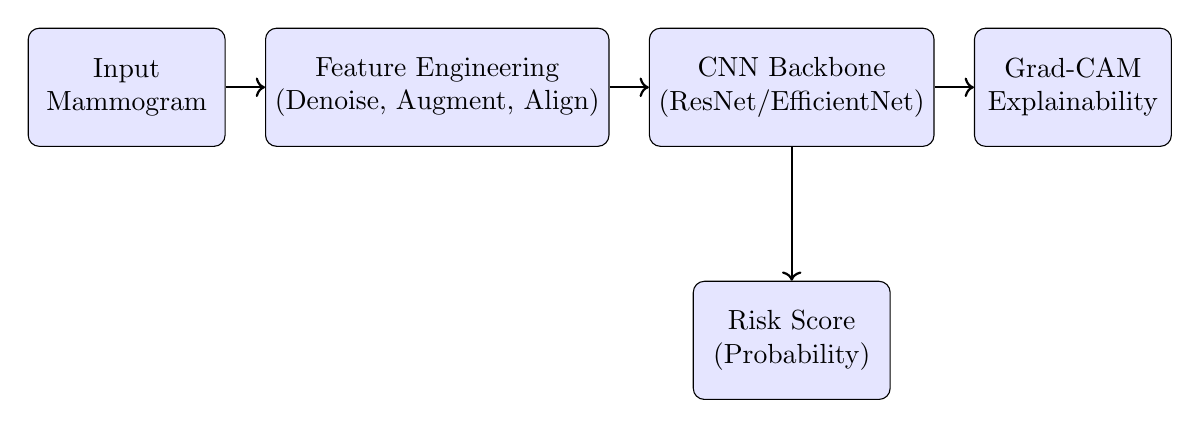
\begin{tikzpicture}[
        node distance=1cm and .5cm,
        box/.style={rectangle, draw=black, fill=blue!10, rounded corners, minimum width=2.5cm, minimum height=1.5cm, align=center},
        arrow/.style={->, thick}
        ]
        
        \node[box] (input) {Input\\Mammogram};
        \node[box, right=of input] (featureeng) {Feature Engineering\\(Denoise, Augment, Align)};
        \node[box, right=of featureeng] (cnn) {CNN Backbone\\(ResNet/EfficientNet)};
        \node[box, right=of cnn] (gradcam) {Grad-CAM\\Explainability};
        \node[box, below=1.7cm of cnn] (output) {Risk Score\\(Probability)};
        
        \draw[arrow] (input) -- (featureeng);
        \draw[arrow] (featureeng) -- (cnn);
        \draw[arrow] (cnn) -- (gradcam);
        \draw[arrow] (cnn) -- (output);
    \end{tikzpicture}
    \caption{System architecture for explainable breast cancer risk prediction using convolutional neural networks (CNNs)~\cite{1} and Grad-CAM~\cite{5}, with feature engineering integrated as a preprocessing stage.}
    \label{fig:system_architecture}
\end{figure}

\subsection{System Architecture Overview}

\subsubsection{Preprocessing Pipeline}
\label{sec:pipeline}
To ensure model robustness, preprocessing standardizes image inputs for consistent downstream processing. Following best practices in mammogram preprocessing~\cite{7,14} and insights from the DDSM dataset~\cite{18}, images are converted to 8-bit grayscale to reduce computational cost while preserving essential tissue detail. Histogram normalization minimizes contrast variability across acquisition devices, aiding generalizability. Each image is resized to 224×224 pixels to match CNN input requirements~\cite{1}, and irrelevant annotations and borders are removed to prevent model bias.

\subsubsection{Model Architecture}
Feature extraction is performed using ResNet-50 or EfficientNet-B0, both known for their strong performance in medical imaging~\cite{1,7}. ResNet-50 offers greater depth and accuracy, while EfficientNet-B0 provides computational efficiency through compound scaling.
Extracted features pass through fully connected layers and terminate in a sigmoid-activated neuron that outputs a cancer risk score. Binary cross-entropy is used as the primary loss function, with focal loss~\cite{2} optionally applied to address class imbalance and increase sensitivity to rare malignancies.

\subsubsection{Explainability and Modular Design}
To improve interpretability, Grad-CAM ~\cite{5} generates heatmaps that highlight regions
contributing most to the prediction, supporting clinical trust, especially in dense or ambiguous cases. Figure~\ref{fig:system_architecture} illustrates the CNN’s dual-path output: risk prediction and
Grad-CAM overlay.

The system is modular by design, allowing future enhancements such as fine-tuning
with Singapore-specific data, integration of patient metadata, or multi-view mammogram
support ~\cite{8}. This ensures adaptability to evolving datasets, clinical needs, and deployment
environments.

\subsection{Dataset Used}
\label{sec:dataset}

This project uses annotated medical images to train and evaluate deep learning models for breast cancer detection. The selected datasets~\cite{cbis_ddsm_kaggle} offer diverse mammographic views essential for building and validating the system’s predictive pipeline.

\subsubsection{Primary Dataset And Adaptation}
The Digital Database for Screening Mammography (DDSM)~\cite{18} serves as the primary dataset. It includes over 2,600 cases, each with four standard views and pathology-verified annotations. Its volume and lesion diversity support robust CNN training for classifying benign and malignant findings.

Although not used in this prototype, the BreaKHis dataset~\cite{19} offers high-resolution histopathological images and is planned for future domain adaptation studies comparing mammograms and tissue slides.

\subsubsection{Local Relevance and Augmentation}
To address regional screening challenges, traits from the Singapore Breast Cancer Cohort~\cite{6} and BreastScreen Singapore~\cite{10} Ísuch as higher dense tissue prevalence and smaller breast volumes are considered. Due to limited access to local imaging data, synthetic augmentation simulates these traits to improve the prototype’s relevance for Singaporean women.

\subsection{Feature Engineering}
\label{subsection:Feature Engineering}

As shown in the System Architecture (Figure~\ref{fig:system_architecture}), feature engineering is a core component of the preprocessing module. It transforms raw mammographic data into a standardized, clinically meaningful format suitable for CNN analysis. Positioned before the CNN backbone, this stage directly impacts prediction accuracy and Grad-CAM quality.

\subsubsection{End-to-End Pipeline}
Figure ~\ref{fig:end_to_end_pipeline} outlines the transformations applied to raw DICOM images before CNN-based feature extraction and classification

\begin{figure}[H]
    \centering
    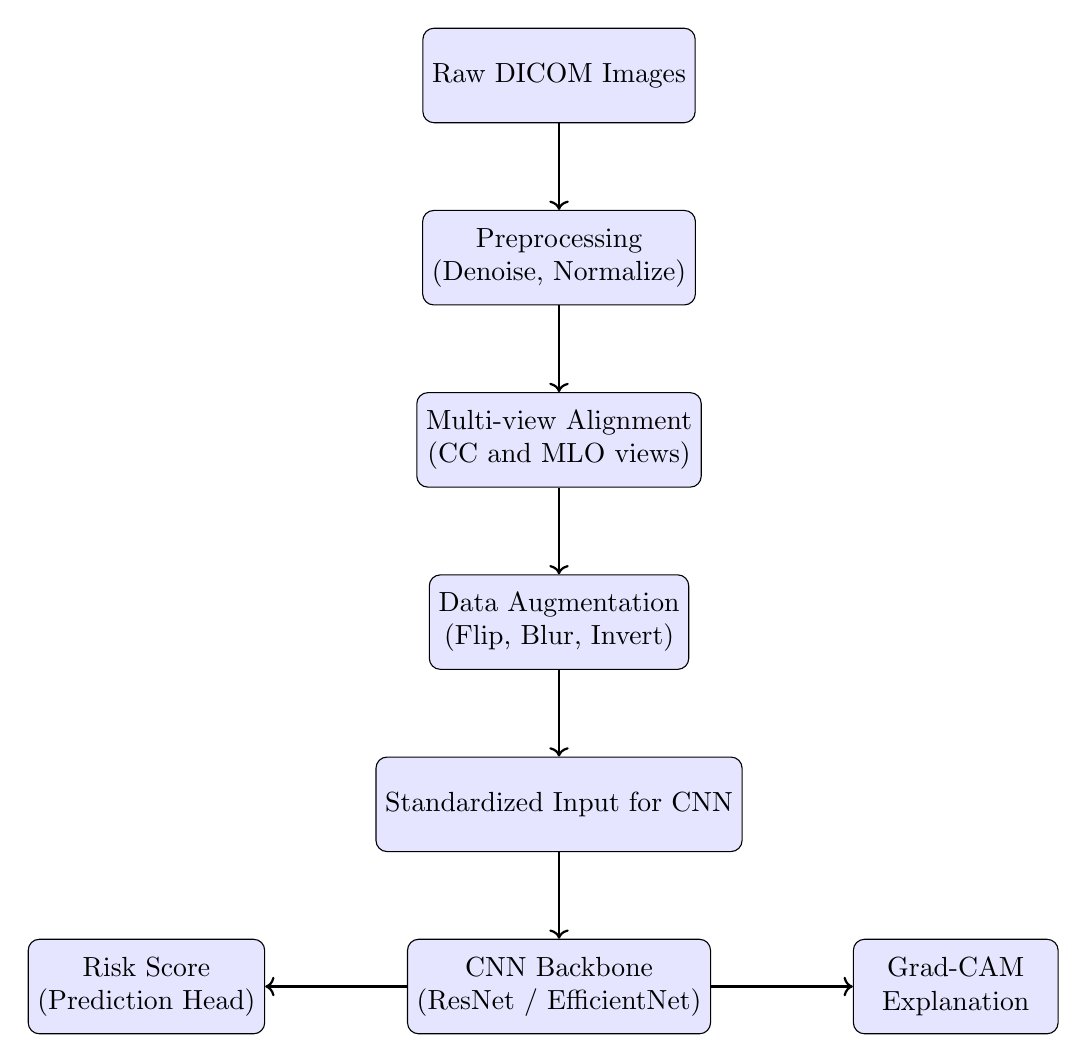
\begin{tikzpicture}[
        node distance=1.1cm and 0.8cm,
        box/.style={rectangle, draw=black, fill=blue!10, rounded corners, minimum width=2.6cm, minimum height=1.2cm, align=center},
        arrow/.style={->, thick}
        ]
        \node[box] (dicom) {Raw DICOM Images};
        \node[box, below=of dicom] (preprocess) {Preprocessing\\(Denoise, Normalize)};
        \node[box, below=of preprocess] (align) {Multi-view Alignment\\(CC and MLO views)};
        \node[box, below=of align] (augment) {Data Augmentation\\(Flip, Blur, Invert)};
        \node[box, below=of augment] (standard) {Standardized Input for CNN};
        \node[box, below=of standard] (cnn) {CNN Backbone\\(ResNet / EfficientNet)};
        \node[box, right=1.8cm of cnn] (gradcam) {Grad-CAM\\Explanation};
        \node[box, left=1.8cm of cnn] (score) {Risk Score\\(Prediction Head)};

        \draw[arrow] (dicom) -- (preprocess);
        \draw[arrow] (preprocess) -- (align);
        \draw[arrow] (align) -- (augment);
        \draw[arrow] (augment) -- (standard);
        \draw[arrow] (standard) -- (cnn);
        \draw[arrow] (cnn) -- (gradcam);
        \draw[arrow] (cnn) -- (score);
    \end{tikzpicture}
    \caption{End-to-end pipeline for breast cancer risk prediction, integrating preprocessing, multi-view alignment, CNN classification, and explainability.}
    \label{fig:end_to_end_pipeline}
\end{figure}

\subsubsection{Design Intent}
This phase aims to improve generalization and sensitivity, especially for dense breast tissue, which is common among Singaporean women. Key transformations include denoising, contrast enhancement, alignment, and augmentation all designed to standardize inputs and simulate clinical variability.

\subsubsection{Preprocessing and Augmentation}

The first step involves enhancing the diagnostic quality of mammograms. Median filtering removes impulse noise while preserving subtle features like microcalcifications. CLAHE (Contrast-Limited Adaptive Histogram Equalization)~\cite{14} improves local contrast, especially in dense tissue. Pixel intensities are then normalized either to $[0,1]$ or z-normalized to support stable training convergence.

Next, augmentation techniques are applied to increase data diversity and reduce overfitting. Geometric transformations such as flipping, cropping, and small-angle rotations (±15°) simulate patient positioning differences. Photometric augmentations (e.g., Gaussian blur and contrast jitter) address scanner inconsistencies. Semantic augmentation via intensity inversion introduces exposure variation and histogram shifts, improving generalizability across imaging devices.

Together, these techniques expand the training distribution and enhance robustness for deployment in diverse clinical environments.

\subsubsection{Multi-View and Domain-Aware Feature Engineering}

Breast screening typically involves two standard views: cranio-caudal (CC) and mediolateral oblique (MLO). Rather than treating these independently, this project adopts a multi-view approach inspired by Geras et al.~\cite{8}, who demonstrated that view fusion improves lesion localization and diagnostic accuracy. CC and MLO views are aligned to maintain anatomical consistency, allowing the model to detect asymmetries and view-specific lesion projections—critical for real-world screening performance.

\begin{figure}[H]
\centering
\includegraphics[width=0.55\textwidth]{images/GerasFig1.png}
\caption{High-resolution mammogram processing via multi-view deep CNNs. Adapted from Geras et al.~\cite{8}.}
\label{fig:geras}
\end{figure}

Domain-specific knowledge is also integrated to improve interpretability and clinical sensitivity. Asymmetry detection is implemented using breast difference maps, which highlight structural discrepancies between left and right breasts. Texture features such as spiculations often linked to malignancy are emphasized using Gabor filters~\cite{20}. Additionally, BI-RADS~\cite{16} density levels are approximated via grayscale histograms and used to weight the loss function. This density-informed stratification gives higher priority to diagnostically challenging dense cases, reflecting the clinical realities of Singaporean screening programs.

Collectively, these strategies enhance both diagnostic accuracy and interpretability, aligning the system with its goal of delivering a culturally adapted, clinically grounded AI solution for breast cancer risk prediction.

\subsection{Algorithm Selection}
\subsubsection{Model Architecture Choices}
Model architecture is selected based on its ability to balance diagnostic accuracy, computational efficiency, and interpretability. ResNet-50 is used as the primary benchmark due to its proven effectiveness in a range of medical imaging applications~\cite{1,7}. To evaluate trade-offs in performance and resource requirements, two alternative models are also considered. EfficientNet-B0 is included for its compound scaling strategy, which achieves strong accuracy while maintaining a low parameter count. This makes it especially suitable for deployment in hospital systems or on edge devices with limited computational power. Additionally, a custom shallow CNN trained from scratch is introduced, based on the findings of Raghu et al.~\cite{2}, who noted that transfer learning from natural image datasets such as ImageNet may not always provide meaningful improvements for medical domains. This model is used to explore whether a locally optimized architecture offers advantages in screening contexts specific to Singaporean women.

\subsubsection{Training Configuration}
Model training is optimized using the Adam optimizer with a cyclical learning rate schedule. To mitigate overfitting, dropout layers are applied after the final dense layer, and early stopping is used with a patience of 10 epochs to prevent unnecessary training once validation performance stabilizes.

\subsection{Evaluation Metrics}
\label{sec:evaluation_metrics}
Model performance is assessed using metrics aligned with clinical relevance, screening effectiveness, and robustness to class imbalance. These reflect the needs of early breast cancer detection, particularly in dense tissue and low-resource settings.

\subsubsection{Primary Performance Metrics}
AUC (Area Under the ROC Curve) is the primary metric, as it captures the model’s ability to distinguish benign from malignant cases across thresholds~\cite{1}. Sensitivity and specificity are reported to assess detection and false positive rates. Sensitivity is prioritized to avoid missed malignancies, especially common in dense tissue~\cite{6}. The F1-score balances precision and recall—especially relevant in imbalanced datasets where accuracy can mislead.

\subsubsection{Explainability Assessment}
Explainability is assessed using Grad-CAM, which produces heatmaps showing the image regions most influential to predictions. These are overlaid on mammograms and—where feasible—reviewed by domain experts to assess alignment with expected tumor locations. This supports clinical trust, regulatory compliance, and interpretability.

\begin{figure}[H]
\centering
\includegraphics[width=0.8\textwidth]{images/gradcam_sample.png}
\caption{Grad-CAM visualizations showing model attention over mammograms. Red indicates regions of high diagnostic interest.}
\end{figure}

\subsubsection{Risk Stratification and Validation}
For risk stratification, patients are ranked based on predicted risk scores and divided into deciles. Clinical utility is assessed through additional metrics including cumulative incidence in the top decile, hazard ratios, and calibration curves.

To ensure generalizability, the training process includes 5-fold stratified cross-validation. The final performance evaluation is conducted on a held-out test set to prevent data leakage and overfitting.

In conclusion, the evaluation strategy for this project combines both standard and domain-specific techniques to ensure clinical relevance and technical robustness. The inclusion of Grad-CAM, dense tissue-aware model training, and local context simulation ensures that the resulting system is aligned with the diagnostic realities faced in Southeast Asia, particularly in under-screened populations.

\subsection{Work Plan and Project Timeline}

This project follows a structured timeline spanning from July to early September 2024, divided into four main phases to manage complexity, reduce risk, and ensure timely delivery. The planning was informed by a top-down decomposition of tasks based on project requirements, module interdependencies, and key submission milestone. Each phase was allocated based on task duration, estimated workload.

\begin{enumerate}
    \item \textbf{Project Conceptualising:} This phase focuses on understanding the problem domain, reviewing prior work, and preparing early deliverables (e.g., proposal video, literature review). Front-loading research activities ensures a strong theoretical foundation for later implementation.

    \item \textbf{Project Planning and Design:} Here, the system architecture, dataset choices, and evaluation methods are formalized. Time is also allocated for early prototyping to identify technical feasibility and refine scope before development.

    \item \textbf{Development and Testing:} The longest phase, this includes model training, iterative testing, and evaluation. Tasks are sequenced to allow progressive model improvements while maintaining checkpoints for early validation. This modular approach reduces integration risk.

    \item \textbf{Final Sprint:} Reserved for final evaluation, report writing, and video presentation. A buffer period is also included (Week 25) to manage unexpected delays, ensuring submission readiness without compromising quality.
\end{enumerate}

Figure~\ref{fig:gantt} presents the Gantt chart

\begin{figure}[H]
    \centering
    \includegraphics[width=\textwidth]{images/PPR_GanttChart.png}
    \caption{Project Gantt chart showing planned activities from July to September 2024, divided into phases of research, design, development, and reporting.}
    \label{fig:gantt}
\end{figure}

\vspace{2em}
\noindent\textbf{Word count:} 1815

%-------------Feature Prototype Page-------------
\newpage
\section{Feature Prototype}
\subsection{Development Strategy}

This section outlines the current implementation progress l, based on the modular pipeline and objectives established in \hyperref[chapter3]{Chapter 3} (Project Design).

The system comprises four modular stages: (1) data preprocessing, (2) model training, (3) Grad-CAM visualization, and (4) evaluation. Each is implemented as a Jupyter notebook in the project repository: \href{https://github.com/justinlim00/FYP-Overview25/tree/main/FYP%20Project/FYP%20Project%20Code%20V1/notebooks}{GitHub repository}.

\subsubsection{Module Implementation Sequence}
The decision to implement these modules first was driven by their foundational role in validating the project’s technical feasibility. Preprocessing was prioritized to standardize input image dimensions, enforce class balance, and eliminate artifacts, ensuring consistency for downstream model training. A custom CNN was then implemented to serve as the system’s initial classifier. This model incorporated regularization techniques and mechanisms to address class imbalance, directly contributing to Objective 1 (Model Accuracy). Establishing a working baseline classifier was essential before introducing more advanced components such as transfer learning or domain adaptation.

\subsubsection{Robustness Considerations}
To address Objective 2 (Robustness), stratified dataset splitting and class-weighted training were used to improve model performance on underrepresented subgroups, particularly malignant and high-density breast tissue cases. During evaluation, threshold tuning was applied to emphasize sensitivity a critical metric in screening systems aimed at early cancer detection.

\subsubsection{Explainability Features}
In support of {Objective 3 (Explainability)}, Grad-CAM was integrated to produce attention heatmaps, helping clinicians interpret the model’s predictions. This interpretability layer not only aids in validation but also builds trust in AI-assisted diagnostic workflows by providing visual evidence for decision-making.

Modules were developed in dependency order: preprocessing, modeling, visualization, then evaluation. This ensures an operational pipeline and simplifies integration of future enhancements like pretrained models or dashboards.


\subsection{Implemented Modules}
The system was developed in a staged, dependency-driven order to ensure a functional pipeline from the outset. Data preprocessing was prioritized to standardize inputs, followed by model training, interpretability, and finally, evaluation. This sequence aligns with the overall system architecture and the objectives outlined in \hyperref[chapter1]{Chapter 1}

\begin{enumerate}
    \item Data preprocessing must precede all modeling tasks.
    \item Training a working baseline model is a prerequisite for meaningful evaluation or comparison.
    \item Visualization tools (Grad-CAM) were developed early to ensure that model interpretability (Objective 2) could be validated in parallel with model accuracy.
\end{enumerate}

This prioritization ensures that the foundational system works end-to-end, allowing later additions (e.g., pretrained models, dashboard UI) to be integrated without reengineering the core pipeline.


\subsubsection{01\_preprocessing.ipynb}

This module establishes a standardized input pipeline to ensure consistent image formatting and balanced class distributions. The CBIS-DDSM dataset~\cite{18} was selected for its curated, biopsy-confirmed mammograms, making it suitable for model training and evaluation.

Following established preprocessing practices~\cite{7}, input images were converted to grayscale to reduce redundant color channels while preserving tissue structure. Each image was resized to $224 \times 224$ pixels to support compatibility with CNN architectures like ResNet and EfficientNet, and to enable efficient batch training.

The preprocessing script is modular, supporting reuse across experiments. It includes configurable parameters for future enhancements, such as augmentation via rotation and contrast normalization—planned for the next development phase.



\vspace{0.5em}

\subsubsection{02\_model\_training.ipynb}

This module implements the core classification component of the system using a custom Convolutional Neural Network (CNN). The model was selected for its balance between interpretability, computational efficiency, and suitability for binary classification tasks in medical imaging~\cite{17}. The model accepts $224 \times 224$ grayscale inputs and comprises two convolutional blocks with increasing filter sizes (32, then 64), each followed by ReLU activation and max pooling to capture spatial features efficiently. The extracted features are then flattened and passed through a Dense layer with 128 ReLU-activated units, followed by a Dropout layer (rate = 0.5) to reduce overfitting. The final output layer consists of a single sigmoid-activated neuron, optimized for binary classification.

Training is conducted using the binary cross-entropy loss function and the Adam optimizer with a learning rate of 0.001. A batch size of 32 is used, and early stopping with a patience of 5 epochs is applied to prevent overfitting and conserve computational resources. Initial validation accuracy plateaued near 80\%, but divergence between training and validation losses in later epochs suggests some degree of overfitting. To address this, planned improvements include adding batch normalization, adjusting learning rate schedules, and introducing more robust data augmentation strategies in the final implementation phase.

To address class imbalance in CBIS-DDSM, Keras’s class weight parameter was used to upweight malignant samples, enhancing sensitivity crucial to Objective 1.

This model forms the diagnostic core of the system, enabling downstream Grad-CAM and evaluation tools (e.g., ROC and confusion matrices). It also serves as a baseline for testing pretrained models and comparing architectures.

A key innovation was the use of post-training threshold tuning to optimize the precision–recall trade-off. Table~\ref{tab:threshold_metrics} summarizes performance across thresholds.

\begin{table}[H]
\centering
\caption{Precision, Recall, and F1-Score at Different Thresholds}
\label{tab:threshold_metrics}
\begin{tabular}{lccc}
\toprule
Threshold & Precision & Recall & F1-Score \\
\midrule
0.2 & 0.32 & 0.88 & 0.47 \\
0.3 & 0.40 & 0.77 & 0.53 \\
0.5 & 0.55 & 0.45 & 0.49 \\
\bottomrule
\end{tabular}
\end{table}

Threshold 0.3, offering the best F1 and high recall, aligns with the clinical goal of minimizing missed malignancies. At this operating point, the model achieved 77.05\% sensitivity, 40.4\% precision, and an F1-score of 53.0\%. The ROC AUC was 0.5046, indicating weak overall discriminative power and highlighting the need for comparative models and further optimization in the next development phase.

\subsubsection{03\_gradcam\_visualization.ipynb}

This module implements Gradient-weighted Class Activation Mapping (Grad-CAM) to visualize which regions of a mammogram contributed most to the model’s classification decisions, directly addressing Objective 2 (Explainability). A custom Grad-CAM function was developed using Keras, allowing fine control over gradient computation and activation extraction. Heatmaps are computed by backpropagating gradients from the output layer to selected convolutional layers, and overlaid onto grayscale input images to generate interpretable visual cues.

To improve visual clarity, percentile clipping is applied to enhance contrast in the resulting heatmaps. A modular and reusable design was adopted instead of off-the-shelf implementations to provide flexibility in selecting convolutional layers and customizing gradient normalization strategies. This aids tuning for dense tissue cases and cross-model comparisons

\begin{figure}[H]
\centering
\includegraphics[width=0.9\textwidth]{images/gradcam_grid.png}
\caption{Sample Grad-CAM overlay grid (Benign vs Malignant)}
\label{fig:gradcam_grid}
\end{figure}

Figure~\ref{fig:gradcam_grid} presents Grad-CAM overlays on four representative cases. While the visualizations consistently highlight dense or textured regions, they occasionally fail to localize precisely on tumour sites. This indicates that the model may be focusing on general density or morphological cues rather than directly identifying malignancy, highlighting an area for further tuning and validation.

\subsubsection{04\_Evaluation.ipynb}
Preliminary evaluation of the trained CNN model yielded the following results:

\begin{table}[H]
\centering
\caption{Evaluation Metrics on Test Set}
\begin{tabular}{lr}
\toprule
Metric & Score \\
\midrule
Accuracy & 0.4412 \\
Precision & 0.4039 \\
Sensitivity (Recall) & 0.7705 \\
Specificity & 0.2133 \\
F1-Score & 0.5300 \\
AUC & 0.5046 \\
\bottomrule
\end{tabular}
\end{table}

Table 2 reflects a strong sensitivity (77.05\%) but poor specificity, affirming the threshold trade-off decision. This prioritization of sensitivity is clinically motivated, aiming to reduce missed cancers. The AUC value of 0.5046 confirms that the model is performing only marginally better than random guessing.

\begin{figure}[H]
\centering
\includegraphics[width=0.45\textwidth]{images/confusion_matrix.png}
\caption{Confusion Matrix (Threshold = 0.3)}
\end{figure}
Figure 2 confirms this bias, with a large number of false positives contributing to the low specificity. This outcome is a direct result of the decision to shift the threshold in favor of higher recall.

\begin{figure}[H]
\centering
\includegraphics[width=0.5\textwidth]{images/roc_curve.png}
\caption{ROC Curve with AUC = 0.5046}
\end{figure}
Figure 2 shows the trade-off: high false positives and low specificity, due to prioritizing recall.

\subsection{Improvements and Next Steps}
\label{improvements}

\subsubsection{Architecture Benchmarking}
To fulfill the objectives outlined in Section 1.3 and align with the system architecture detailed in Chapter 3, several tasks have been scheduled for the final development phase. First, to address Objective 3 regarding architecture benchmarking, additional models such as pretrained ResNet50 and VGG16 will be implemented. These models will be evaluated using the same data splits and performance metrics as the current prototype to determine whether transfer learning improves discriminability in mammography classification tasks.

\subsubsection{Grad-CAM Enhancements}
Grad-CAM outputs will also be enhanced to improve the precision of interpretability (Objective 2). Current heatmaps tend to highlight broad regions without reliably localizing tumour structures. Planned improvements include scaling adjustments, percentile-based contrast boosting, and experimenting with visualizations from earlier convolutional layers to capture finer texture features that are often clinically relevant.

\subsubsection{Evaluation Pipeline Finalization}
In addition, the evaluation pipeline will be finalized by migrating manual metric computations into a dedicated evaluation notebook. This notebook will automate the generation of confusion matrices, ROC curves, and metric tables across various classification thresholds, improving reproducibility and ensuring alignment with Section 3.6 on evaluation strategy.

\subsubsection{Threshold Optimization}
Threshold optimization will also be formalized. Since the current model performs best at a threshold of 0.3, future iterations will apply systematic methods such as grid search or the Youden index to identify the optimal classification threshold. These results will be presented in tabular form for comparison and justification.

\subsubsection{Stratified Evaluation by Breast Density}
Lastly, stratified evaluation by breast density will be introduced to assess model robustness in diagnostically challenging scenarios. Although the CBIS-DDSM dataset includes density metadata, stratified analysis has not yet been conducted. This planned step is essential to Objective 2, as it evaluates the model’s effectiveness in high-density cases common among Singaporean women, thereby improving clinical validity and alignment with real-world screening contexts.


\vspace{2em}
\noindent\textbf{Word count:} 1500


%-------------Appendices Page-------------
\newpage
\section{Appendices}

\begin{figure}[H]
    \centering
    \includegraphics[width=\textwidth]{images/lit1table2.png}
    \caption{Performance comparison between the Tyrer-Cuzick model and deep learning models across subgroups. Adapted from [1].}
    \label{fig:lit1table2}
\end{figure}

\begin{figure}[H]
    \centering
    \includegraphics[width=0.9\textwidth]{images/hybrid_risk_by_density.png}
    \caption{Cancer incidence across density groups and hybrid risk scores. Adapted from ~cite{1}.}
    \label{fig:hybrid_density}
\end{figure}

\begin{figure}[H]
    \centering
    \includegraphics[height=0.7\textheight]{images/lit1_roc_auc.png}
    \caption{ROC curves comparing Tyrer-Cuzick, image-only DL, and hybrid DL models. Adapted from [1].}
    \label{fig:lit1roc}
\end{figure}

\begin{figure}[H]
    \centering
    \includegraphics[width=0.85\textwidth]{images/ShenFig2.png}
    \caption{CNN-generated detection probabilities on mammograms. Adapted from [7].}
    \label{fig:shen2019}
\end{figure}


\begin{figure}[H]
    \centering
    \includegraphics[width=\textwidth]{images/gradcam_sample.png}
    \caption{Example of Grad-CAM heatmaps overlaid on mammograms, highlighting regions associated with high-risk predictions. Adapted from [5].}
    \label{fig:gradcam}
\end{figure}

\begin{figure}[H]
    \centering
    \includegraphics[width=\textwidth]{images/lit2table7.png}
    \caption{Comparison of pretrained vs. randomly initialized CNNs in medical imaging tasks. Adapted from [2].}
    \label{fig:lit2table7}
\end{figure}

%-------------References Page-------------
\newpage
\section{References}
\begin{thebibliography}{99}

    \bibitem{1}
    A. Yala, C. Lehman, T. Schuster, T. Portnoi, and R. Barzilay. 2019. A Deep Learning Mammography based Model for Improved Breast Cancer Risk Prediction. \textit{Radiology} 292, 1 (2019), 60–66. \url{https://pubs.rsna.org/doi/pdf/10.1148/radiol.2019182716}
    
    \bibitem{2}
    M. Raghu, C. Zhang, J. Kleinberg, and S. Bengio. 2019. Transfusion: Understanding Transfer Learning for Medical Imaging. In \textit{Proc. NeurIPS 2019}, 3342–3352. \url{https://proceedings.neurips.cc/paper/2019/file/eb1e78328c46506b46a4ac4a1e378b91-Paper.pdf}
    
    \bibitem{3}
    T. Ching, D. S. Himmelstein, B. K. Beaulieu-Jones, et al. 2018. Opportunities and obstacles for deep learning in biology and medicine. \textit{Nature Reviews Genetics} 19 (2018), 141–158. \url{https://royalsocietypublishing.org/doi/full/10.1098/rsif.2017.0387}
    
    \bibitem{4}
    V. Cheplygina, M. de Bruijne, and J. P. W. Pluim. 2019. Not-so-supervised: A survey of semi-supervised, multi-instance, and transfer learning in medical image analysis. \textit{Medical Image Analysis} 54 (2019), 280–296. \url{https://arxiv.org/pdf/1804.06353}
    
    \bibitem{5}
    R. R. Selvaraju, et al. 2017. Grad-CAM: Visual Explanations from Deep Networks via Gradient-based Localization. In \textit{Proc. ICCV}, 618–626. \url{https://openaccess.thecvf.com/content_ICCV_2017/papers/Selvaraju_Grad-CAM_Visual_Explanations_ICCV_2017_paper.pdf}
    
    \bibitem{6}
    W. Y. Chau, G. H. Lim, Y. L. Ng, et al. 2021. Breast density and breast cancer risk in Asian women: Evidence from the Singapore Breast Screening Programme. \textit{Cancer Epidemiology} 74 (2021), 101987. \url{https://pmc.ncbi.nlm.nih.gov/articles/PMC5160133/}
    
    \bibitem{7}
    L. Shen, L. R. Margolies, J. H. Rothstein, et al. 2019. Deep learning to improve breast cancer detection on screening mammography. \textit{Scientific Reports} 9, 1 (2019), 12495. \url{https://www.nature.com/articles/s41598-019-48995-4}
    
    \bibitem{8}
    K. J. Geras, S. Wolfson, Y. Shen, et al. 2017. High-resolution breast cancer screening with multi-view deep convolutional neural networks. \textit{arXiv preprint arXiv:1703.07047}. \url{https://arxiv.org/abs/1703.07047}
    
    \bibitem{9}
    H. J. Kim, E. Y. Ko, C. Kim, W. Han, and W. K. Moon. 2018. Applying Data-driven Imaging Biomarker in Mammography for Breast Cancer Screening: Preliminary Study. \textit{Scientific Reports} 8, 1 (2018), 12210. \url{https://www.ncbi.nlm.nih.gov/pmc/articles/PMC5807343/}
    
    \bibitem{10}
    National Registry of Diseases Office. 2022. \textit{Singapore Cancer Registry Annual Report 2022}. \url{https://www.nrdo.gov.sg/docs/librariesprovider3/default-document-library/scr-ar-2022_web-report.pdf?sfvrsn=a9eb8c10_1}

    \bibitem{11}
    S. M. McKinney, M. Sieniek, V. Godbole, J. Godwin, N. Antropova, H. Ashrafian, et al. 2020. International evaluation of an AI system for breast cancer screening. \textit{Nature}, 577 (2020), 89–94. \url{https://www.nature.com/articles/s41586-019-1799-6}

    \bibitem{12}
    Zebra Medical Vision. 2021. Zebra’s AI1 Mammography Solutions. \url{https://www.zebra-med.com/}

    \bibitem{13}
    N. Salim, J. L. Andersson, A. Nordenskjöld, H. Svensson, K. Törnberg, and K. Zackrisson. 2024. Artificial intelligence for breast cancer screening in a real-world, population-based setting: cohort study of 58,000 mammograms. \textit{Nature Medicine}, (2024). \url{https://www.nature.com/articles/s41591-024-03061-0}

    \bibitem{14}
    J. Shen, L. Margolies, J. Rothstein, E. Fluder, R. McBride, and W. Sieh. 2019. Deep Learning to Improve Breast Cancer Detection on Screening Mammography. \textit{Scientific Reports} 9 (2019), 12495. \url{https://www.nature.com/articles/s41598-019-48995-4}

    \bibitem{14}
    K. Zuiderveld. 1994. Contrast Limited Adaptive Histogram Equalization. In P. S. Heckbert (Ed.), \textit{Graphics Gems IV}, 474–485. Academic Press. \url{https://doi.org/10.1016/B978-0-08-050755-2.50065-6}

    \bibitem{16}
    American College of Radiology. 2013. Breast Imaging Reporting and Data System (BI-RADS). \textit{ACR BI-RADS Atlas, Breast Imaging Reporting and Data System}. 5th Edition. American College of Radiology.

    \bibitem{17}
    K. He, X. Zhang, S. Ren, and J. Sun. 2016. Deep Residual Learning for Image Recognition. In \textit{Proc. CVPR}, 770–778. \url{https://doi.org/10.1109/CVPR.2016.90}

    \bibitem{18}
    M. Heath, K. Bowyer, D. Kopans, R. Moore, and W. P. Kegelmeyer. 2000. The Digital Database for Screening Mammography. In \textit{Proc. 5th International Workshop on Digital Mammography}, 212–218. \url{http://www.eng.usf.edu/cvprg/Mammography/Database.html}

    \bibitem{19}
    I. A. Spanhol, L. S. Oliveira, C. Petitjean, and L. Heutte. 2016. A dataset for breast cancer histopathological image classification. \textit{IEEE Transactions on Biomedical Engineering}, 63, 7 (2016), 1455–1462. \url{https://doi.org/10.1109/TBME.2015.2496264}

    \bibitem{20}
    J. Daugman. 1985. Uncertainty relation for resolution in space, spatial frequency, and orientation optimized by two-dimensional visual cortical filters. \textit{Journal of the Optical Society of America A}, 2, 7 (1985), 1160–1169. \url{https://doi.org/10.1364/JOSAA.2.001160}

    \bibitem{cbis_ddsm_kaggle}
    Awsaf49. CBIS-DDSM Breast Cancer Image Dataset. Kaggle. \url{https://www.kaggle.com/datasets/awsaf49/cbis-ddsm-breast-cancer-image-dataset?resource=download}

    \bibitem{github_fyp}
    Justin Lim. 2025. \textit{FYP-Overview25 GitHub Repository – Breast Cancer Detection Prototype Notebooks}. Retrieved from \url{https://github.com/justinlim00/FYP-Overview25/tree/main/FYP%20Project/FYP%20Project%20Code%20V1/notebooks}
    
    \end{thebibliography}
    
\end{document}